\documentclass[a4paper,12pt,oneside]{report}

\usepackage[utf8]{inputenc}
\usepackage[T1]{fontenc}
\usepackage{geometry}
\usepackage{setspace}
\usepackage{graphicx}
\usepackage{float}
\usepackage{longtable}
\usepackage{array}
\usepackage{enumitem}
\usepackage{xcolor}
\usepackage{hyperref}
\usepackage{tikz}
\usetikzlibrary{arrows.meta,positioning,shapes.geometric}
\usepackage{url}
\usepackage[nottoc]{tocbibind}

\geometry{margin=1in}
\setstretch{1.2}

\begin{document}

% ===================== TITLE PAGE =====================
\begin{titlepage}
    \centering
    \vspace*{1cm}

    {\Large \textbf{EduRate: Professor Rating and Performance Analytics System}\par}
    \vspace{0.6cm}
    {\large Project Report\par}
    \vspace{1.2cm}

    A report submitted for the course named \textbf{Project-I (CSE3021)}\par

    \vspace{1.5cm}
    
\includegraphics[width=4cm]{screenshots/iiit-manipur.png}
    \vspace{1.2cm}

    Submitted By\par
    \vspace{0.3cm}
    {\Large \textbf{MOHIT GORA}}\\
    Roll No: \textbf{230101056}

    \vspace{0.9cm}
    Supervised By\par
    \vspace{0.3cm}
    {\Large \textbf{Dr. Sanasam Chanu Inunganbi}}

    \vfill
    {\large Department Of Computer Science And Engineering\\
    Indian Institute of Information Technology Senapati, Manipur\\
    Submission Date: \underline{\hspace{3cm}}}
\end{titlepage}

% ===================== DECLARATION =====================
\chapter*{Declaration}
In this submission, I have expressed my idea in my own words, and I have adequately cited and referenced any ideas or words that were taken from another source. I also declare that I adhere to all principles of academic honesty and integrity and that I have not misrepresented or falsified any ideas, data, facts, or sources in this submission. If any violation of the above is made, I understand that the institute may take disciplinary action. Such a violation may also engender disciplinary action from the sources which were not properly cited or permission not taken when needed.

\vspace{1cm}\hspace{8.2cm} MOHIT GORA \\
\vspace{0.5cm}\hspace{8.2cm} 230101056 \\
\vspace{0.5cm} DATE: \underline{\hspace{3cm}}

\newpage

% ===================== ABSTRACT =====================
\chapter*{Abstract}
EduRate is a full-stack web application designed to improve transparency and quality in academic feedback systems. The platform offers separate interfaces for students, professors, and administrators. Students can rate professors, provide feedback, post doubts, and use a performance prediction feature. Professors can view feedback and respond to student doubts. Administrators can monitor faculty performance and send email-based performance reports.

The system uses HTML, CSS, JavaScript, Node.js, Express.js, MySQL, JWT authentication, bcrypt hashing, and Chart.js for data visualization. The platform also includes role-based access control, trend analysis, and structured performance history. EduRate provides a practical model for digital, data-driven quality monitoring in educational institutions.

\newpage

% ===================== ACKNOWLEDGEMENT =====================
\chapter*{Acknowledgement}
I express my sincere gratitude to \textbf{Dr. Sanasam Chanu Inunganbi} for valuable guidance, encouragement, and support during this project. I am also thankful to the Department Of Computer Science And Engineering, Indian Institute of Information Technology Senapati, Manipur, for providing the opportunity and resources to complete this work.

\tableofcontents
\listoffigures
\newpage

\chapter{Introduction}
\section{Overview}
EduRate is a full-stack, role-based academic platform developed to improve transparency and quality in faculty feedback and student support workflows. The system provides a unified dashboard through which students can rate professors, submit constructive feedback, post doubts, and use a performance prediction module. Professors can review feedback insights and respond to student doubts, while administrators can monitor teaching performance trends and communicate reports.

\section{Background and Motivation}
In many institutions, feedback collection remains periodic and largely manual. Such systems produce delayed insights, lower student engagement, and limited actionability for academic departments. A modern institution requires a system that can:
\begin{enumerate}[label=\Alph*., leftmargin=1.5em]
    \item collect structured feedback continuously instead of once-per-semester,
    \item provide transparent and comparable performance indicators for faculty,
    \item support day-to-day student-professor interaction through doubt resolution,
    \item help administrators review and act on performance data quickly.
\end{enumerate}
EduRate is motivated by these institutional requirements and by the availability of lightweight web technologies capable of delivering a practical and scalable solution.

\section{Problem Statement}
Existing feedback portals usually operate as isolated forms with minimal analytics. They often lack strict role separation, real-time dashboards, unified communication channels, and actionable outcomes such as rankings, trend analysis, and targeted reporting. As a result, performance monitoring is delayed and opportunities for academic improvement are frequently missed.

\section{Objectives}
\begin{enumerate}[leftmargin=1.5em]
    \item Design and implement secure authentication with role-based access control.
    \item Build a professor rating and textual feedback module with aggregated metrics.
    \item Implement a doubt management workflow for posting and answering queries.
    \item Provide a student-side performance predictor with historical trend visibility.
    \item Create an admin analytics panel with individual and bulk performance email reporting.
    \item Maintain modular code organization for maintainability and future extension.
\end{enumerate}

\section{Scope}
The current scope includes student, professor, and admin workflows in a single application intended for institute-level deployment. The project covers authentication, rating operations, doubt handling, performance prediction, analytics visualization, and report communication. Future expansion may include richer AI analytics, periodic report exports, and advanced predictive modeling.

\section{Significance}
EduRate provides measurable value to all stakeholders:
\begin{enumerate}[label=\Alph*., leftmargin=1.5em]
    \item \textbf{Students:} Better participation, feedback expression, and preparation insights.
    \item \textbf{Professors:} Structured visibility of ratings and student interaction records.
    \item \textbf{Administration:} Data-supported monitoring and communication for quality assurance.
\end{enumerate}

\section*{Chapter Summary}
This chapter introduced the project context, institutional motivation, and specific objectives addressed by EduRate. It established the scope and significance of the platform for students, professors, and administrators, thereby defining the foundation for subsequent technical chapters.


\chapter{Literature Survey}
\section{Existing Systems}
Conventional professor feedback systems in higher education are commonly form-based and batch-processed at semester end. While these systems collect basic ratings, they usually do not provide interactive dashboards, faculty engagement tracking, or integrated communication workflows.

\section{Identified Gaps}
\begin{enumerate}[label=\Alph*., leftmargin=1.5em]
    \item delayed analysis due to offline or end-semester processing,
    \item limited administrative visibility into ongoing faculty performance,
    \item low integration between rating systems and student support workflows,
    \item no mechanism for real-time trend visualization and ranking,
    \item no student-centric academic prediction support in the same platform.
\end{enumerate}

\section{Proposed Contribution}
EduRate addresses these gaps through a unified, role-based web platform that integrates:
\begin{enumerate}[label=\Alph*., leftmargin=1.5em]
    \item secure login and authorization for multiple stakeholders,
    \item professor ratings with actionable textual feedback,
    \item doubt posting and response workflow with usage control,
    \item performance analytics for both student and administrative views,
    \item email-based faculty reporting for institutional communication.
\end{enumerate}

\section{Comparative Perspective}
Compared to standard feedback portals, EduRate introduces continuous analytics, engagement features, and administrative action support. This improves the practical utility of feedback data and transforms it from static records into a decision-support resource.

\section*{Chapter Summary}
This chapter reviewed existing feedback system patterns, identified major operational and analytical gaps, and justified the contribution of EduRate as an integrated, role-aware, and decision-support-oriented platform.


\chapter{Requirement Engineering}
\section{Functional Requirements}
\begin{enumerate}[leftmargin=1.5em]
    \item User registration and login with credential validation.
    \item Role support for student, professor, and admin users.
    \item Professor directory with profile details and metadata.
    \item Star-based rating with textual feedback submission.
    \item Doubt posting by students with daily limit enforcement.
    \item Doubt answer workflow for professors.
    \item Student performance prediction module with history retention.
    \item Trend chart visualization for prediction outcomes.
    \item Admin dashboard with teacher performance indicators.
    \item Individual and bulk email reporting from admin panel.
\end{enumerate}

\section{Non-Functional Requirements}
\begin{enumerate}[label=\Alph*., leftmargin=1.5em]
    \item \textbf{Security:} JWT-based session validation and bcrypt password hashing.
    \item \textbf{Performance:} Fast dashboard rendering and efficient API response.
    \item \textbf{Usability:} Clean navigation and role-specific interface.
    \item \textbf{Reliability:} Persistent storage in MySQL.
    \item \textbf{Scalability:} Modular backend APIs and frontend components.
\end{enumerate}

\section{User Roles}
\begin{enumerate}[label=\Alph*., leftmargin=1.5em]
    \item \textbf{Student:} Rate professors, post doubts, use prediction module.
    \item \textbf{Professor:} View feedback and answer doubts.
    \item \textbf{Admin:} View analytics and send performance reports.
\end{enumerate}

\section{Use Case Analysis}
\subsection*{Use Case 1: Authentication}
\textbf{Actors:} Student, Professor, Admin\\
\textbf{Precondition:} User has registered credentials.\\
\textbf{Main Flow:} The user submits login details, the system verifies credentials, and the user is redirected according to role.

\subsection*{Use Case 2: Rating Submission}
\textbf{Actor:} Student\\
\textbf{Precondition:} Student is logged in.\\
\textbf{Main Flow:} The student selects a professor, submits rating and feedback, and the system stores the record and updates aggregates.

\subsection*{Use Case 3: Doubt Handling}
\textbf{Actors:} Student, Professor\\
\textbf{Precondition:} Both are authenticated.\\
\textbf{Main Flow:} The student posts a doubt, the professor reviews and answers it, and the system updates the doubt status.

\subsection*{Use Case 4: Performance Reporting}
\textbf{Actor:} Admin\\
\textbf{Precondition:} Admin is logged in.\\
\textbf{Main Flow:} The admin reviews performance metrics and sends individual or bulk performance emails to professors.

\section{Data Requirements}
Core data entities include users, professors, ratings, doubts, sessions, and email logs. Relationships enforce traceability of who submitted feedback, who answered doubts, and which professor each performance metric belongs to.

\section*{Chapter Summary}
This chapter formalized the requirement baseline for EduRate across functional, non-functional, and role-specific expectations. It also documented representative use cases and data entities required for robust implementation and verification.


\chapter{System Design}
\section{Introduction}
This chapter presents the logical and structural design of EduRate. It describes how system components interact, how data flows across modules, and how core entities are organized in storage.

\section{Architecture Overview}
EduRate follows a client-server architecture with a web frontend, REST APIs, and a MySQL backend.

\begin{figure}[H]
\centering
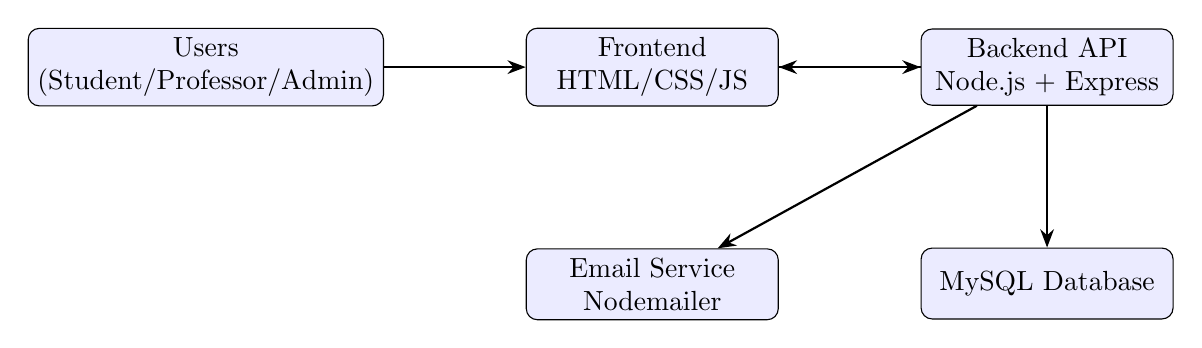
\begin{tikzpicture}[
  node distance=1.8cm and 1.8cm,
  box/.style={draw, rounded corners, minimum width=3.2cm, minimum height=0.9cm, align=center, fill=blue!8},
  arr/.style={-Stealth, thick}
]
\node[box] (users) {Users\\(Student/Professor/Admin)};
\node[box, right=of users] (frontend) {Frontend\\HTML/CSS/JS};
\node[box, right=of frontend] (api) {Backend API\\Node.js + Express};
\node[box, below=of api] (db) {MySQL Database};
\node[box, below=of frontend] (email) {Email Service\\Nodemailer};

\draw[arr] (users) -- (frontend);
\draw[arr] (frontend) -- (api);
\draw[arr] (api) -- (db);
\draw[arr] (api) -- (email);
\draw[arr] (api) -- (frontend);
\end{tikzpicture}

\caption{System Architecture Diagram}
\end{figure}
\noindent\textit{This diagram presents the high-level architecture of EduRate. It shows how users interact with the frontend, backend services, and database for core workflows.}

\subsection*{Architecture Components}
\begin{enumerate}[label=\Alph*., leftmargin=1.5em]
    \item \textbf{Presentation Layer:} Browser-based UI for students, professors, and admins.
    \item \textbf{Application Layer:} Express APIs for authentication, ratings, doubts, predictions, and admin actions.
    \item \textbf{Data Layer:} MySQL schema with relational tables and analytical views.
    \item \textbf{External Service Layer:} Email communication via Nodemailer.
\end{enumerate}

\section{DFD Level 0 (Context Diagram)}
\begin{figure}[H]
\centering
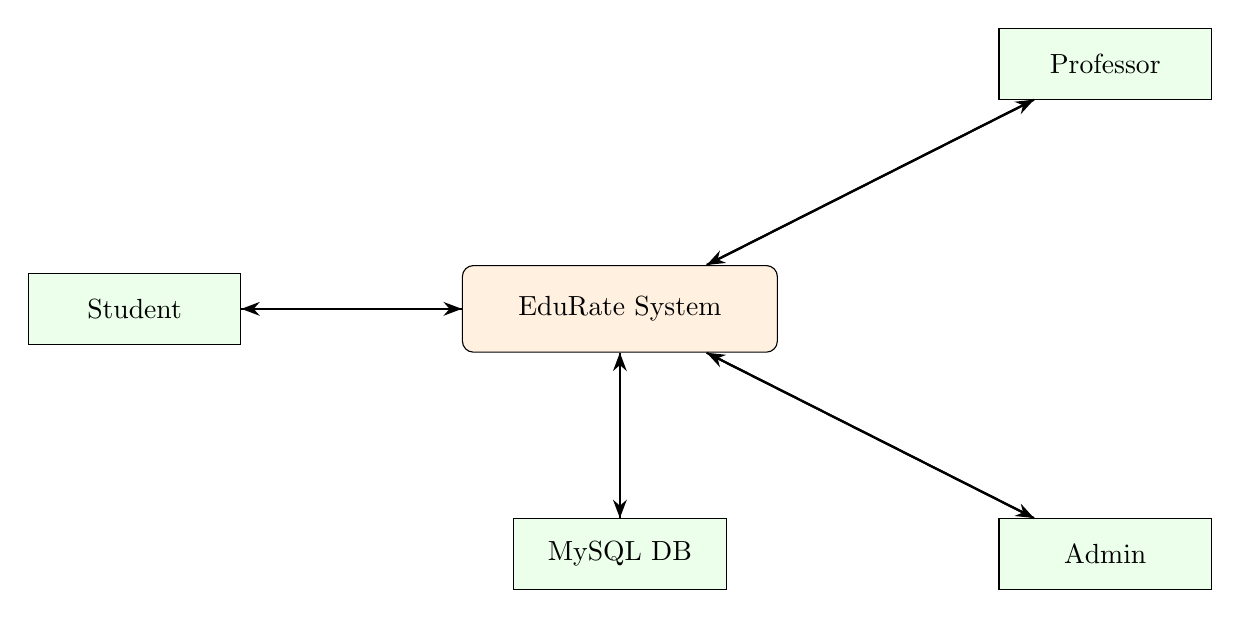
\begin{tikzpicture}[
  node distance=2.1cm and 2.8cm,
  ext/.style={draw, minimum width=2.7cm, minimum height=0.9cm, fill=green!8, align=center},
  proc/.style={draw, rounded corners, minimum width=4cm, minimum height=1.1cm, fill=orange!12, align=center},
  arr/.style={-Stealth, thick}
]
\node[proc] (sys) {EduRate System};
\node[ext, left=of sys] (student) {Student};
\node[ext, above right=of sys] (prof) {Professor};
\node[ext, below right=of sys] (admin) {Admin};
\node[ext, below=of sys] (db) {MySQL DB};

\draw[arr] (student) -- (sys);
\draw[arr] (sys) -- (student);
\draw[arr] (prof) -- (sys);
\draw[arr] (sys) -- (prof);
\draw[arr] (admin) -- (sys);
\draw[arr] (sys) -- (admin);
\draw[arr] (sys) -- (db);
\draw[arr] (db) -- (sys);
\end{tikzpicture}

\caption{DFD Level 0}
\end{figure}
\noindent\textit{This context-level DFD highlights the external entities that interact with the system. It summarizes major data exchange between users and the EduRate platform.}

\subsection*{DFD Level 0 Description}
At the context level, EduRate exchanges requests and responses with three external entities (student, professor, and admin) while persisting and retrieving records from the database.

\section{DFD Level 1}
\begin{figure}[H]
\centering
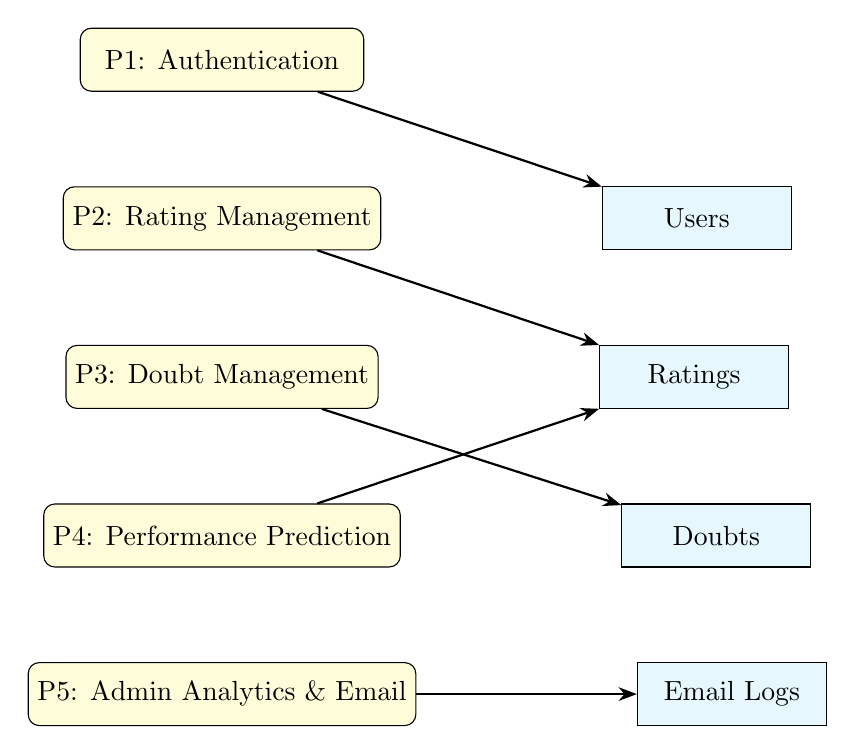
\begin{tikzpicture}[
  node distance=1.2cm and 1.6cm,
  proc/.style={draw, rounded corners, minimum width=3.6cm, minimum height=0.8cm, fill=yellow!15, align=center},
  store/.style={draw, minimum width=2.4cm, minimum height=0.8cm, fill=cyan!10, align=center},
  arr/.style={-Stealth, thick}
]
\node[proc] (p1) {P1: Authentication};
\node[proc, below=of p1] (p2) {P2: Rating Management};
\node[proc, below=of p2] (p3) {P3: Doubt Management};
\node[proc, below=of p3] (p4) {P4: Performance Prediction};
\node[proc, below=of p4] (p5) {P5: Admin Analytics \& Email};

\node[store, right=2.8cm of p2] (d1) {Users};
\node[store, right=2.8cm of p3] (d2) {Ratings};
\node[store, right=2.8cm of p4] (d3) {Doubts};
\node[store, right=2.8cm of p5] (d4) {Email Logs};

\draw[arr] (p1) -- (d1);
\draw[arr] (p2) -- (d2);
\draw[arr] (p3) -- (d3);
\draw[arr] (p5) -- (d4);
\draw[arr] (p4) -- (d2);
\end{tikzpicture}

\caption{DFD Level 1}
\end{figure}
\noindent\textit{This diagram decomposes the main system into functional processes such as authentication, ratings, doubts, and reporting. It also indicates key data stores used by each process.}

\subsection*{DFD Level 1 Description}
The level-1 decomposition presents major internal processes for authentication, ratings, doubts, prediction, and administrative communication. Each process reads from or updates specific data stores.

\section{DFD Level 2 (Rating and Feedback Process)}
\begin{figure}[H]
\centering
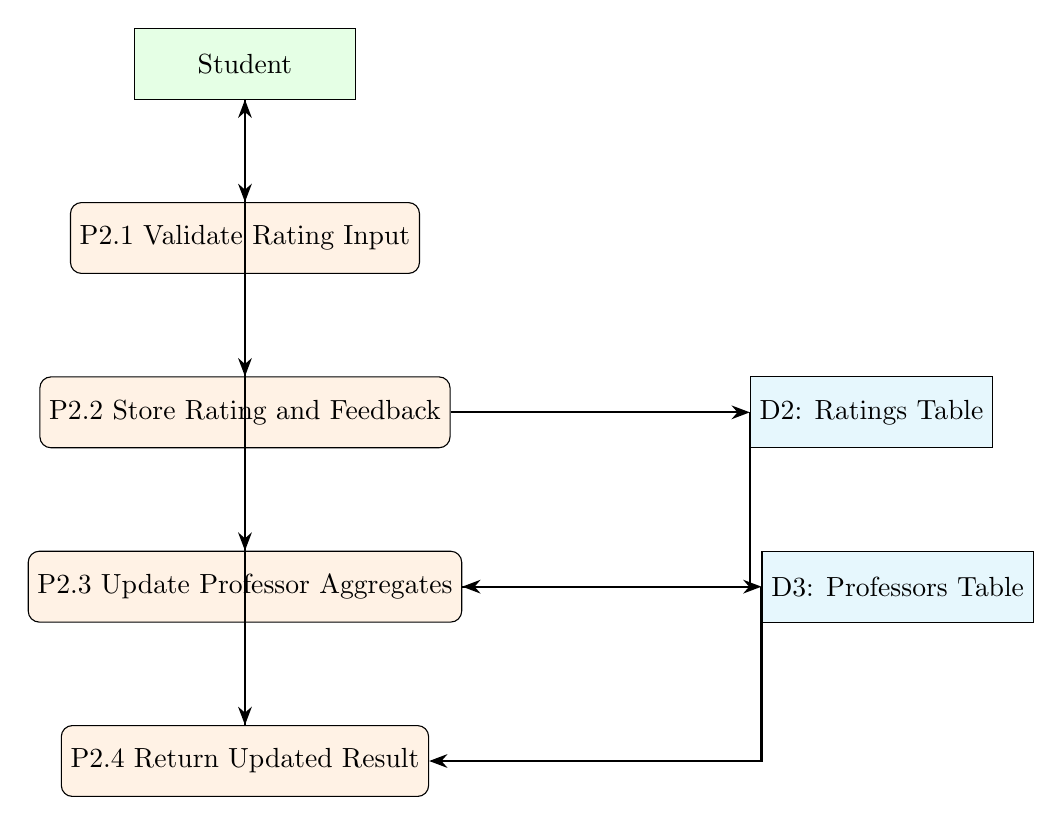
\begin{tikzpicture}[
  node distance=1.3cm and 1.8cm,
  proc/.style={draw, rounded corners, minimum width=4.0cm, minimum height=0.9cm, fill=orange!10, align=center},
  store/.style={draw, minimum width=3.0cm, minimum height=0.9cm, fill=cyan!10, align=center},
  ext/.style={draw, minimum width=2.8cm, minimum height=0.9cm, fill=green!10, align=center},
  arr/.style={-Stealth, thick}
]
\node[ext] (student) {Student};
\node[proc, below=of student] (validate) {P2.1 Validate Rating Input};
\node[proc, below=of validate] (save) {P2.2 Store Rating and Feedback};
\node[proc, below=of save] (aggregate) {P2.3 Update Professor Aggregates};
\node[proc, below=of aggregate] (refresh) {P2.4 Return Updated Result};

\node[store, right=3.8cm of save] (ratings) {D2: Ratings Table};
\node[store, right=3.8cm of aggregate] (profs) {D3: Professors Table};

\draw[arr] (student) -- (validate);
\draw[arr] (validate) -- (save);
\draw[arr] (save) -- (aggregate);
\draw[arr] (aggregate) -- (refresh);
\draw[arr] (refresh) -- (student);

\draw[arr] (save.east) -- (ratings.west);
\draw[arr] (aggregate.east) -- (profs.west);
\draw[arr] (ratings.west) |- (aggregate.east);
\draw[arr] (profs.west) |- (refresh.east);
\end{tikzpicture}

\caption{DFD Level 2}
\end{figure}
\noindent\textit{This level-2 DFD focuses specifically on the rating and feedback pipeline. It captures validation, persistence, aggregate update, and dashboard refresh flow.}

\subsection*{DFD Level 2 Description}
The level-2 model expands the rating process into validation, storage, aggregation update, and dashboard refresh steps. This captures internal logic after student rating submission.

\section{User Journey Diagram}
\begin{figure}[H]
\centering
\begin{tikzpicture}[
  node distance=1.2cm and 1.5cm,
  step/.style={draw, rounded corners, minimum width=4.8cm, minimum height=0.9cm, fill=blue!8, align=center},
  branch/.style={draw, rounded corners, minimum width=4.8cm, minimum height=0.9cm, fill=teal!10, align=center},
  prof/.style={draw, rounded corners, minimum width=4.8cm, minimum height=0.9cm, fill=orange!12, align=center},
  arr/.style={-Stealth, thick}
]
\node[step] (reg) {Student Registration};
\node[step, below=of reg] (login) {User Login};
\node[step, below=of login] (dash) {Student Dashboard Opened};
\node[branch, below left=1.6cm and 3.2cm of dash] (rate) {Open Professor Profile and Submit Rating};
\node[branch, below right=1.6cm and 3.2cm of dash] (doubt) {Post Doubt Query for Professor};
\node[prof, below=2.2cm of doubt] (pdash) {Professor Dashboard Receives Doubt};
\node[prof, below=of pdash] (solve) {Professor Submits Solution/Answer};

\draw[arr] (reg) -- (login);
\draw[arr] (login) -- (dash);
\draw[arr] (dash) -- (rate);
\draw[arr] (dash) -- (doubt);
\draw[arr] (doubt) -- (pdash);
\draw[arr] (pdash) -- (solve);
\end{tikzpicture}

\caption{End-to-End User Journey from Registration to Doubt Resolution}
\end{figure}
\noindent\textit{This flowchart explains the complete operational journey in the application. It begins with registration and login, then shows dashboard usage, rating submission, doubt posting, and professor-side doubt resolution.}

\section{ER Diagram}
\begin{figure}[H]
\centering
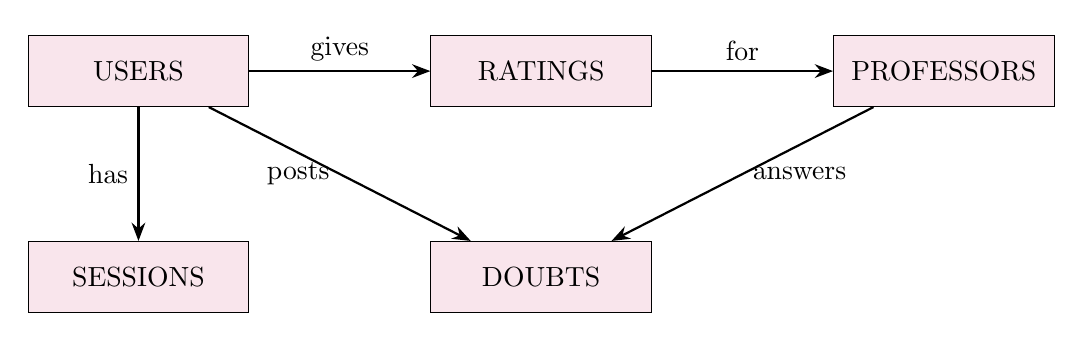
\begin{tikzpicture}[
  node distance=1.7cm and 2.3cm,
  ent/.style={draw, minimum width=2.8cm, minimum height=0.9cm, fill=purple!10, align=center},
  rel/.style={-Stealth, thick}
]
\node[ent] (users) {USERS};
\node[ent, right=of users] (ratings) {RATINGS};
\node[ent, right=of ratings] (profs) {PROFESSORS};
\node[ent, below=of ratings] (doubts) {DOUBTS};
\node[ent, below=of users] (sessions) {SESSIONS};

\draw[rel] (users) -- node[above]{gives} (ratings);
\draw[rel] (ratings) -- node[above]{for} (profs);
\draw[rel] (users) -- node[left]{posts} (doubts);
\draw[rel] (profs) -- node[right]{answers} (doubts);
\draw[rel] (users) -- node[left]{has} (sessions);
\end{tikzpicture}

\caption{Entity Relationship Diagram}
\end{figure}
\noindent\textit{This ER diagram defines the structural relationships among core entities in the EduRate database. It clarifies how user, professor, rating, doubt, and session data are linked.}

\subsection*{ER Design Notes}
The schema ensures one-to-many mappings between users and ratings, professors and ratings, and users and sessions. Doubt records maintain linkage between student queries and professor responses.

\section{Use Case Diagram}
\begin{figure}[H]
\centering
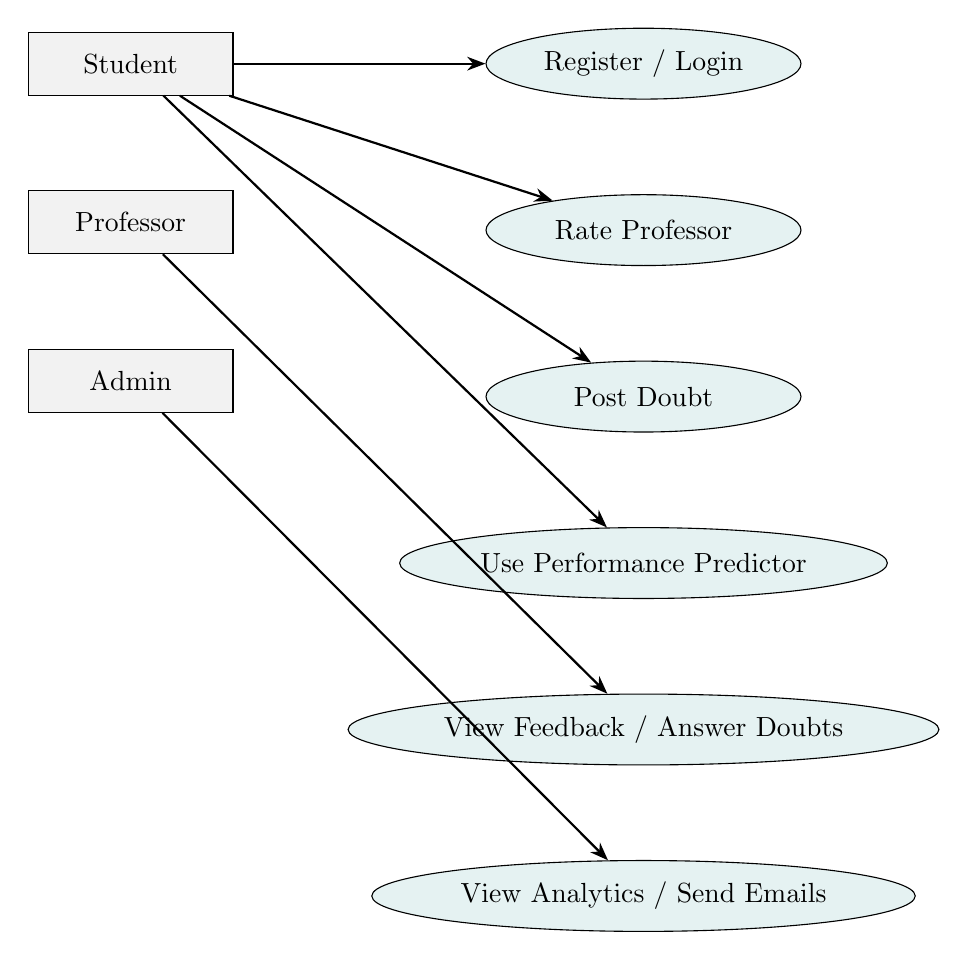
\begin{tikzpicture}[
  node distance=1.2cm and 1.8cm,
  actor/.style={draw, minimum width=2.6cm, minimum height=0.8cm, fill=gray!10, align=center},
  use/.style={draw, ellipse, minimum width=4.0cm, minimum height=0.9cm, fill=teal!10, align=center},
  arr/.style={-Stealth, thick}
]
\node[actor] (student) {Student};
\node[actor, below=of student] (prof) {Professor};
\node[actor, below=of prof] (admin) {Admin};

\node[use, right=3.2cm of student] (u1) {Register / Login};
\node[use, below=of u1] (u2) {Rate Professor};
\node[use, below=of u2] (u3) {Post Doubt};
\node[use, below=of u3] (u4) {Use Performance Predictor};
\node[use, below=of u4] (u5) {View Feedback / Answer Doubts};
\node[use, below=of u5] (u6) {View Analytics / Send Emails};

\draw[arr] (student) -- (u1);
\draw[arr] (student) -- (u2);
\draw[arr] (student) -- (u3);
\draw[arr] (student) -- (u4);
\draw[arr] (prof) -- (u5);
\draw[arr] (admin) -- (u6);
\end{tikzpicture}

\caption{Use Case Diagram}
\end{figure}
\noindent\textit{This use-case view maps responsibilities of students, professors, and administrators. It shows the primary operations available to each role in the application.}

\section{Sequence Diagram (Rating Submission)}
\begin{figure}[H]
\centering
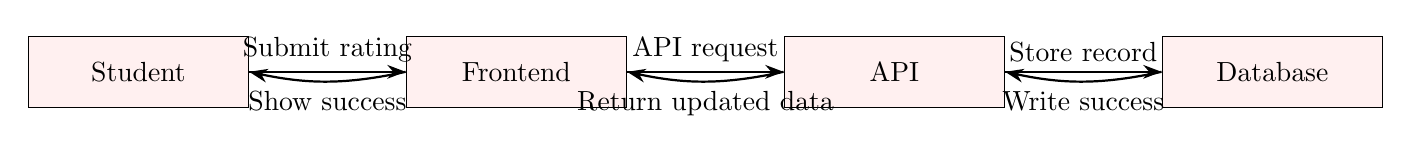
\begin{tikzpicture}[
  lifeline/.style={draw, minimum width=2.8cm, minimum height=0.9cm, fill=red!6, align=center},
  arr/.style={-Stealth, thick}
]
\node[lifeline] (s) at (0,0) {Student};
\node[lifeline] (f) at (4.8,0) {Frontend};
\node[lifeline] (a) at (9.6,0) {API};
\node[lifeline] (d) at (14.4,0) {Database};

\draw[arr] (s.east) -- node[above]{Submit rating} (f.west);
\draw[arr] (f.east) -- node[above]{API request} (a.west);
\draw[arr] (a.east) -- node[above]{Store record} (d.west);
\draw[arr] (d.west) to[bend left=12] node[below]{Write success} (a.east);
\draw[arr] (a.west) to[bend left=12] node[below]{Return updated data} (f.east);
\draw[arr] (f.west) to[bend left=12] node[below]{Show success} (s.east);
\end{tikzpicture}

\caption{Sequence Diagram for Rating Flow}
\end{figure}
\noindent\textit{This sequence diagram illustrates runtime interaction for rating submission. It shows request flow from student interface to backend and database, followed by response propagation.}

\section{Database Design Summary}
Main tables in the schema are:
\begin{enumerate}[label=\Alph*., leftmargin=1.5em]
    \item \texttt{users}
    \item \texttt{professors}
    \item \texttt{ratings}
    \item \texttt{doubts}
    \item \texttt{gifts}
    \item \texttt{sessions}
\end{enumerate}

The design supports normalized storage, referential integrity, and efficient aggregation for analytics views such as top performers and average ratings.
\noindent\textit{The table structure is designed so that each transaction can be traced from user action to persistent storage. This enables both operational reliability and analytics consistency.}

\section*{Chapter Summary}
This chapter presented the architectural and process-level design of EduRate using multiple formal diagrams. It covered DFD levels, ER modeling, sequence logic, and end-to-end user journey so that the complete data and control flow of the system remains clear and auditable.


\chapter{Implementation}
\section{Technology Stack}
\begin{enumerate}[label=\Alph*., leftmargin=1.5em]
    \item Frontend: HTML5, CSS3, JavaScript
    \item Backend: Node.js, Express.js
    \item Database: MySQL
    \item Security: JWT, bcryptjs
    \item Email: Nodemailer
    \item Visualization: Chart.js
\end{enumerate}

\section{Development Environment}
The project was developed using Visual Studio Code, the Node.js runtime, npm for dependency management, and MySQL database tooling. Version control was maintained using Git during feature integration.

\section{Backend Implementation}
The backend is implemented using Express.js with modular routes and middleware. Core implementation points include:
\begin{enumerate}[label=\Alph*., leftmargin=1.5em]
    \item secure login and registration endpoints,
    \item JWT token generation and verification through auth middleware,
    \item performance APIs for teacher ranking and trend retrieval,
    \item admin-only endpoints for individual and bulk email operations.
\end{enumerate}
Database access is handled through MySQL query interfaces, and password security is enforced using bcrypt hashing.

\section{Frontend Implementation}
The frontend is organized into role-aware dashboards and reusable UI sections. Implementation includes:
\begin{enumerate}[label=\Alph*., leftmargin=1.5em]
    \item authentication pages for login and registration,
    \item dashboard tabs for home, professor list, doubts, and analytics,
    \item rating and feedback forms with validation,
    \item performance prediction modal with multi-step input,
    \item chart rendering using Chart.js for trend visualization.
\end{enumerate}

\section{Prediction Logic}
The performance module uses a hybrid strategy:
\begin{enumerate}[label=\Alph*., leftmargin=1.5em]
    \item weighted formula based on study behavior and previous performance,
    \item regression blending using historical entries for better estimation,
    \item final output in the format \textbf{Expected Score: X / 10}.
\end{enumerate}

\section{Error Handling and Validation}
Input validation is implemented at both frontend and backend levels to prevent invalid records. API responses use structured status and message handling to provide clearer user feedback and easier debugging.

\section{Limitations}
The current implementation is optimized for institute-scale deployment; however, it can be further enhanced through advanced model calibration, centralized logging, and deeper historical analytics.

\section*{Chapter Summary}
This chapter described the concrete implementation of the EduRate platform across frontend, backend, and data layers. It also summarized technical choices, validation strategy, prediction logic, and current system limitations for future enhancement planning.


\chapter{Results and Screenshots}
\section{Overview of Results}
This chapter presents interface-level and functional results observed after implementation. The findings confirm that role-based operations, performance analytics, and communication workflows are functioning as intended.

\section{Login Interface}
\begin{figure}[H]
\centering
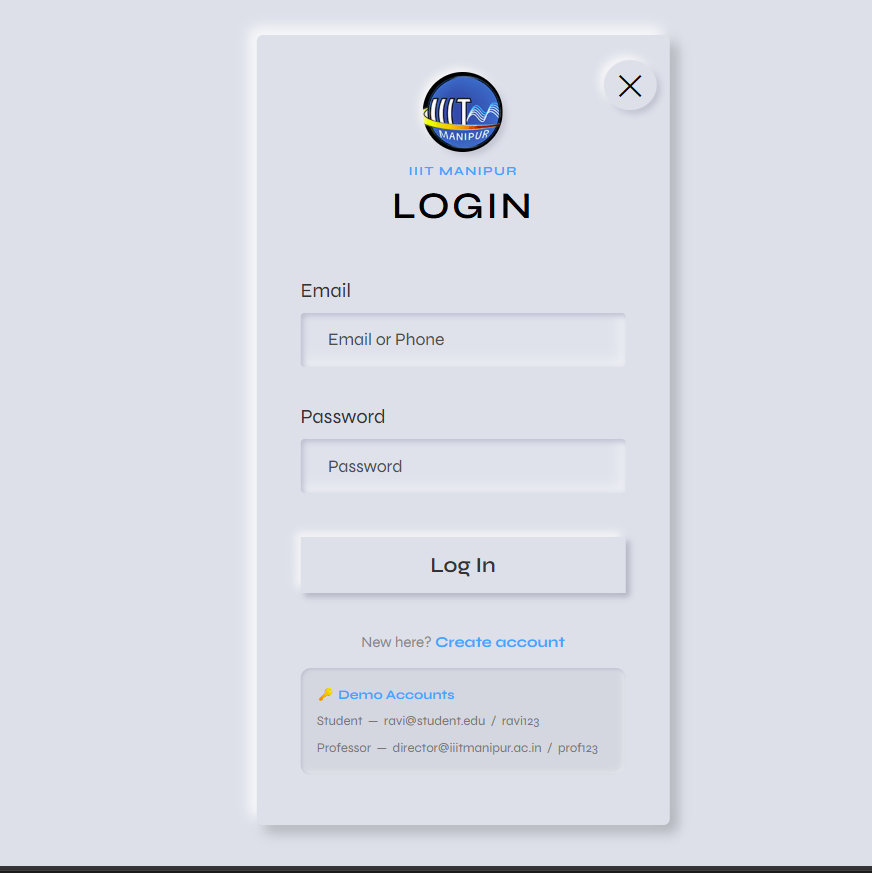
\includegraphics[width=0.9\textwidth]{screenshots/login.png}
\caption{Login Page}
\end{figure}
\noindent\textit{The login interface provides secure access using registered credentials. It acts as the common entry point for all role-based workflows.}

\section{Registration Interface}
\begin{figure}[H]
\centering
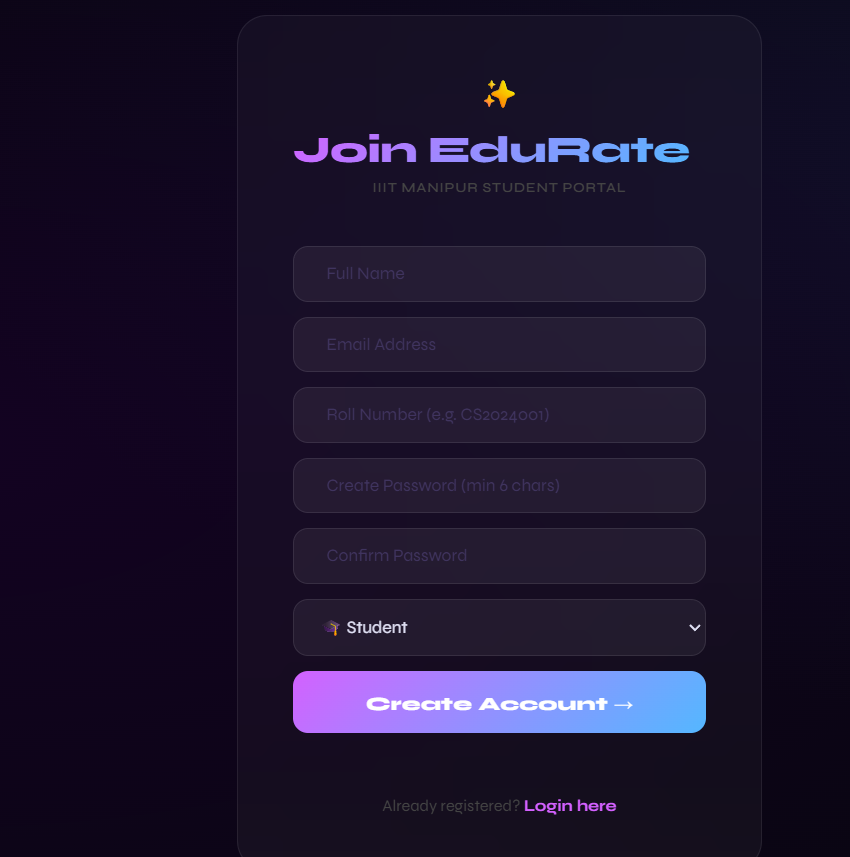
\includegraphics[width=0.9\textwidth]{screenshots/register.png}
\caption{Registration Page}
\end{figure}
\noindent\textit{The registration page captures user details and creates new accounts with role mapping. Input validation ensures completeness and basic data correctness.}

\section{Student Dashboard}
\begin{figure}[H]
\centering
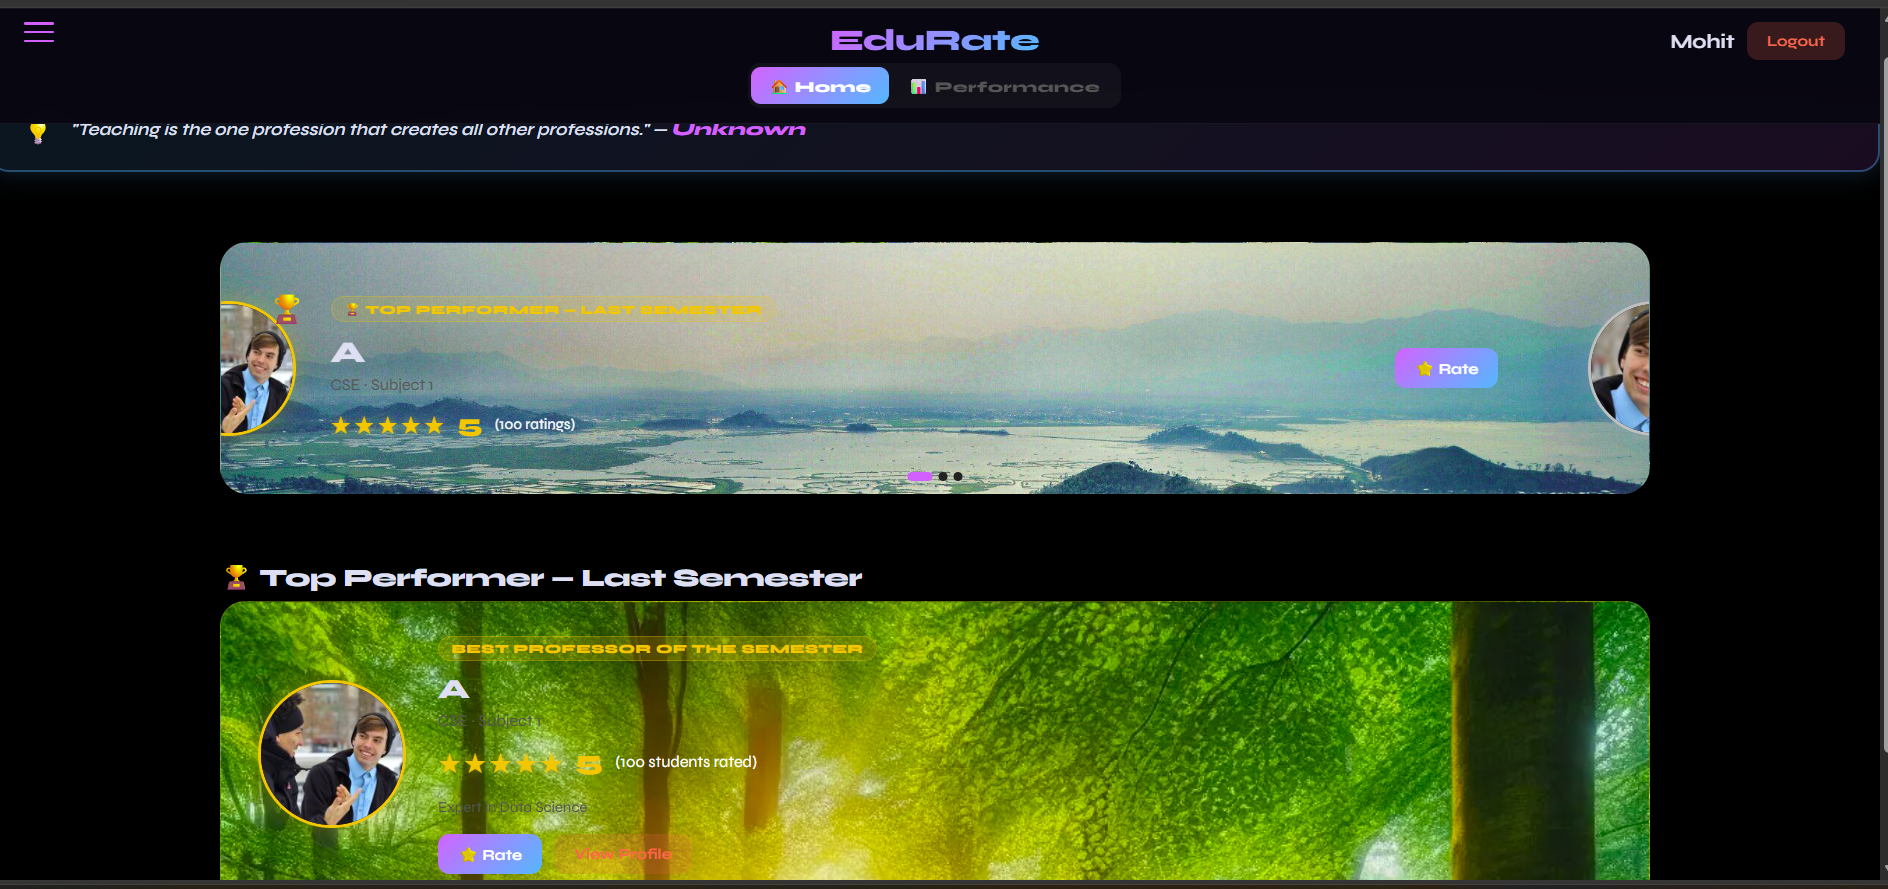
\includegraphics[width=0.95\textwidth]{screenshots/dashboard_student.png}
\caption{Student Dashboard}
\end{figure}
\noindent\textit{The student dashboard consolidates key learning support actions in one place. It offers quick navigation to ratings, doubts, and performance tools.}

\section{Menu Interface}
\begin{figure}[H]
\centering
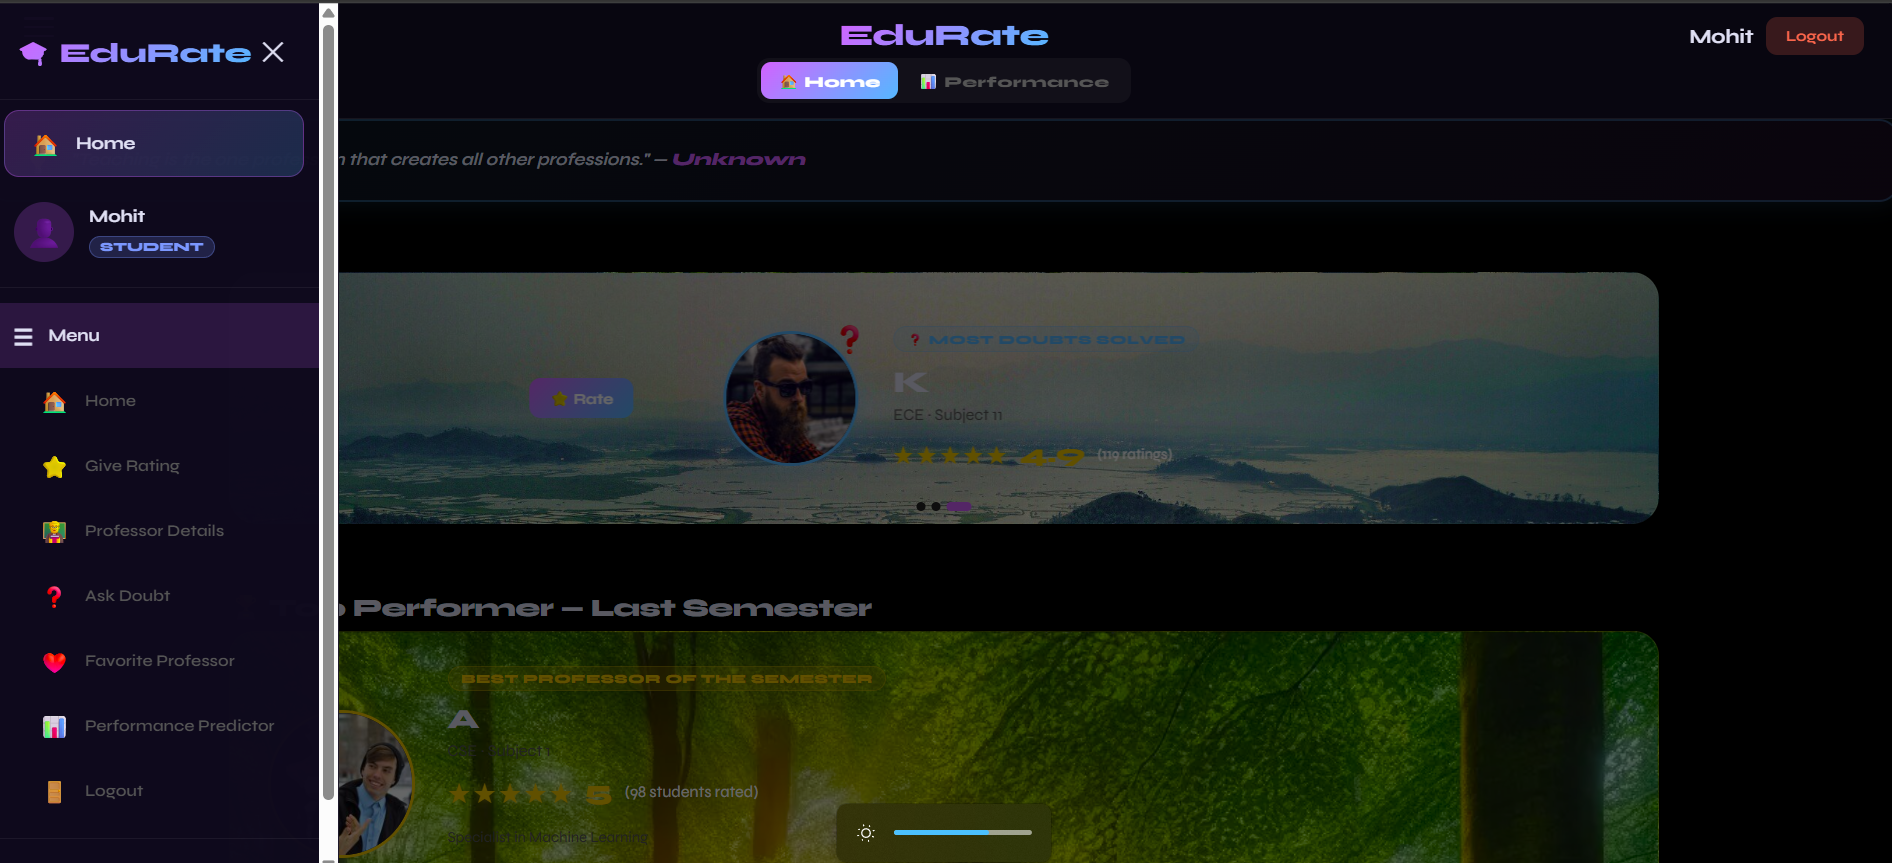
\includegraphics[width=0.95\textwidth]{screenshots/menu.png}
\caption{Dashboard Menu}
\end{figure}
\noindent\textit{The dashboard menu presents organized navigation for role-specific modules. It improves usability by reducing interaction complexity across features.}

\section{Doubt Module}
\begin{figure}[H]
\centering
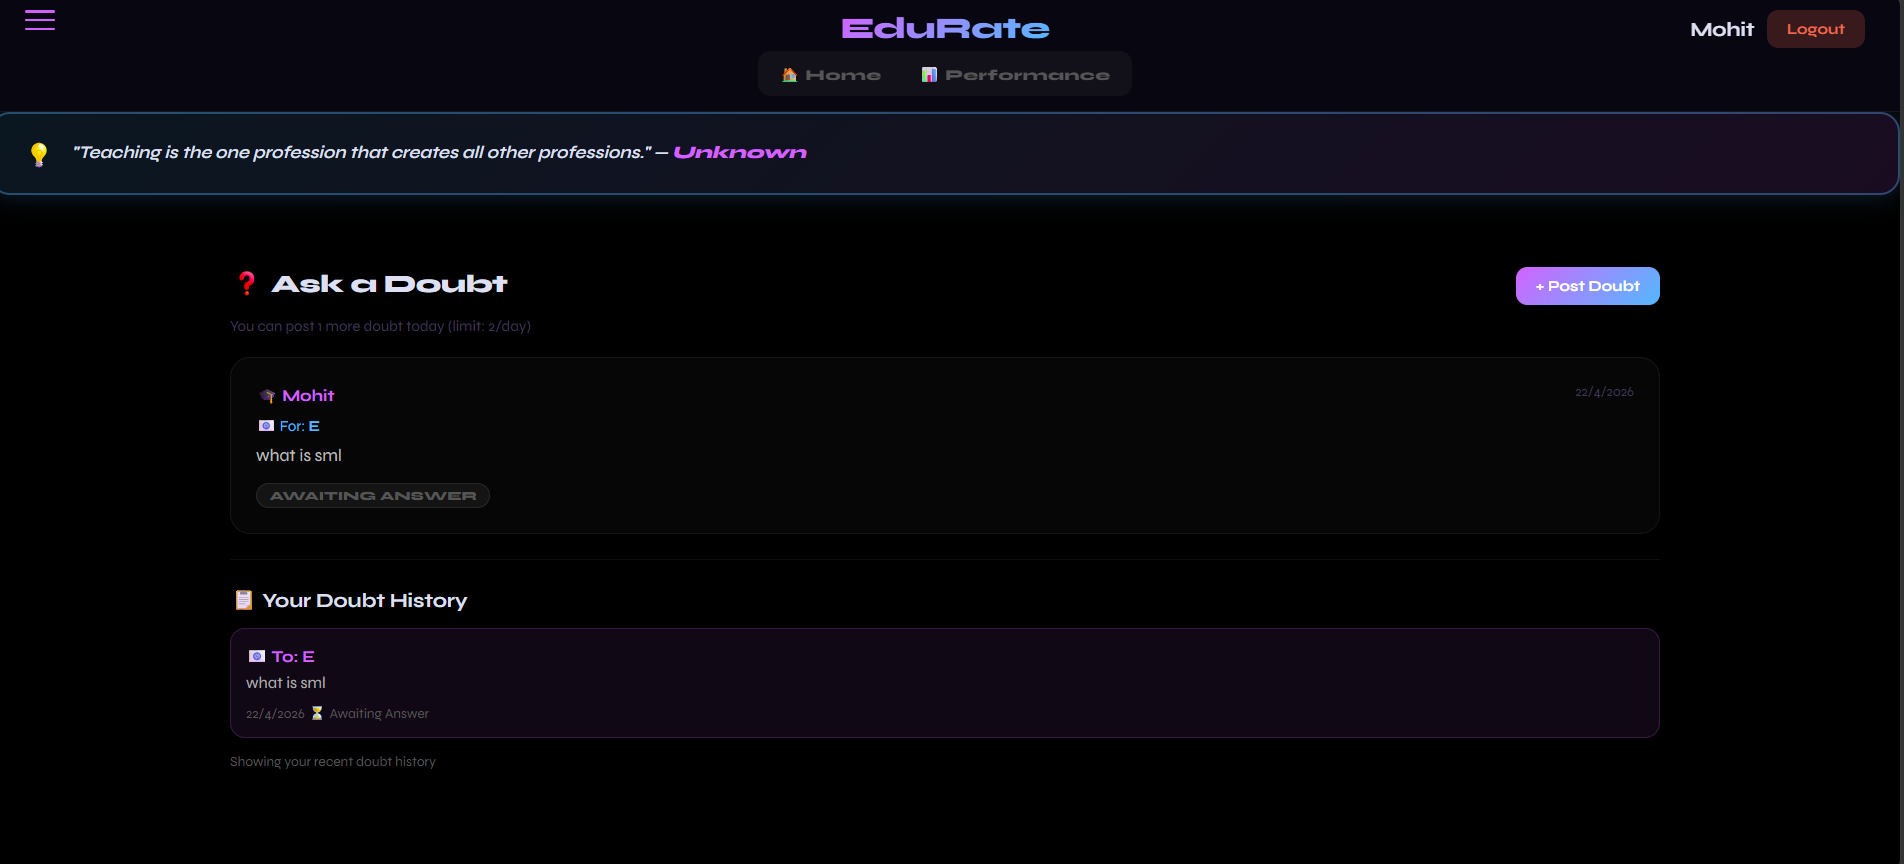
\includegraphics[width=0.95\textwidth]{screenshots/Doubt.png}
\caption{Doubt Posting and Response Module}
\end{figure}
\noindent\textit{This module enables students to post academic queries and receive faculty responses. Daily constraints and status visibility maintain structured interaction.}

\section{Performance Predictor Form}
\begin{figure}[H]
\centering
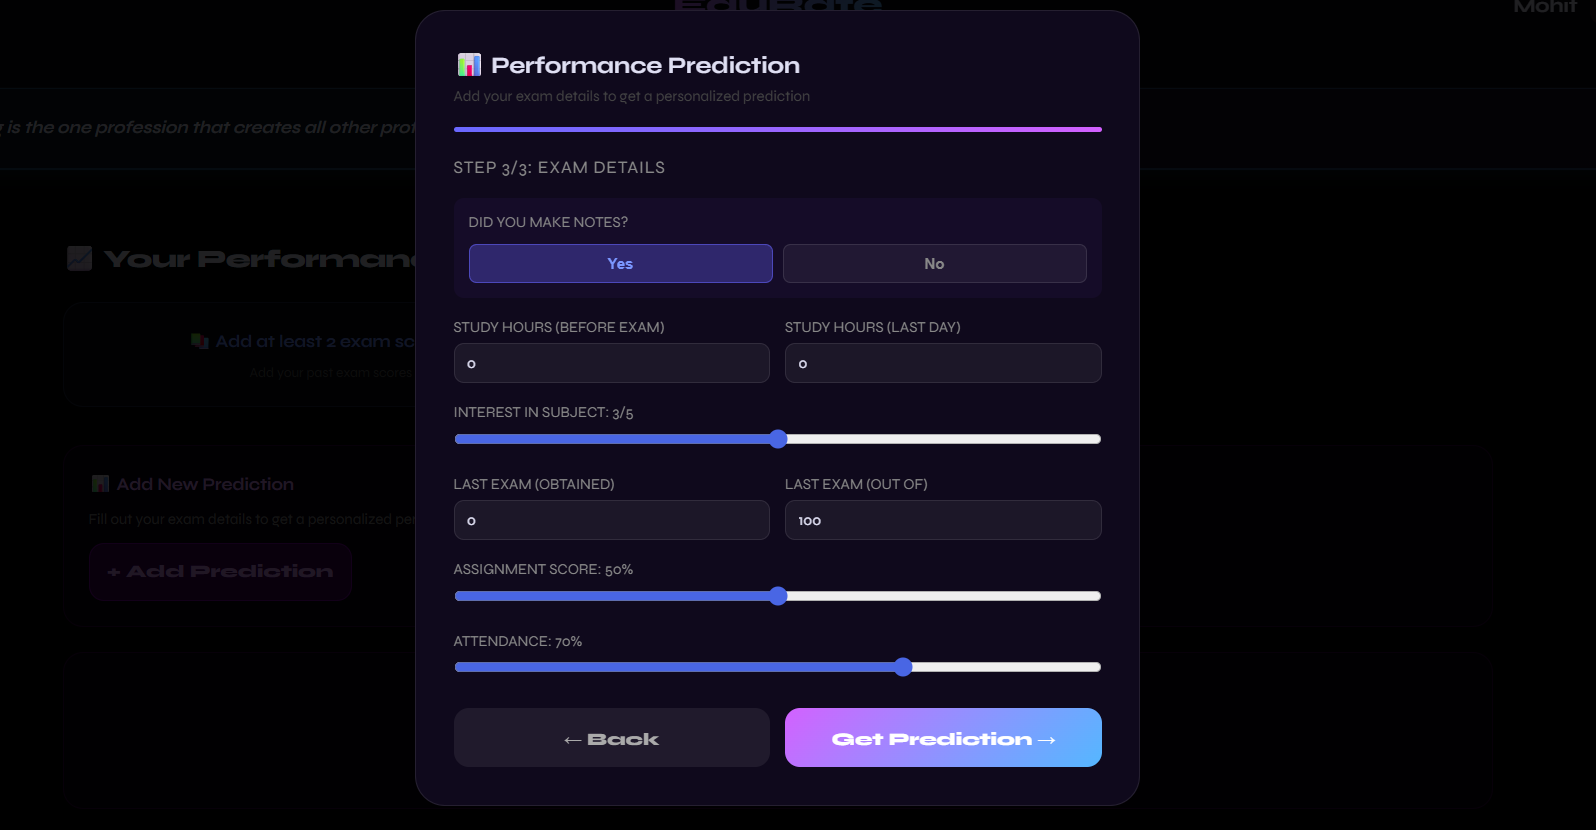
\includegraphics[width=0.95\textwidth]{screenshots/performance_prediction.png}
\caption{Performance Prediction Input Form}
\end{figure}
\noindent\textit{The prediction form collects multi-factor study and assessment inputs. These values are used to estimate expected academic performance.}

\section{Prediction Output}
\begin{figure}[H]
\centering
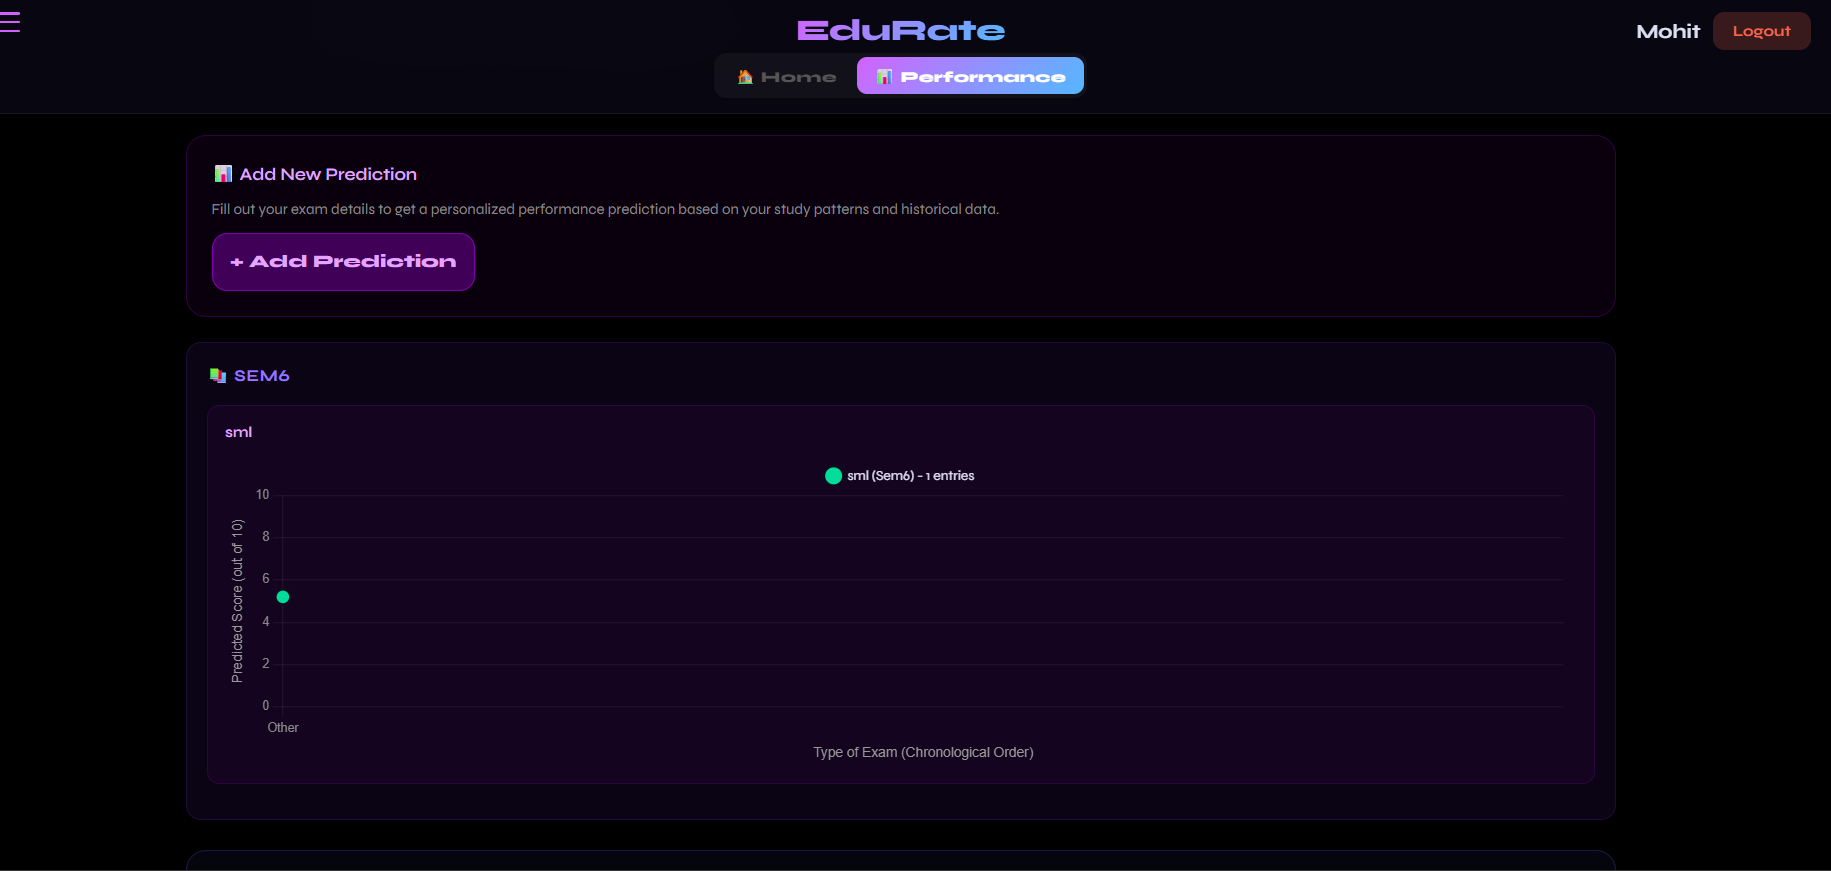
\includegraphics[width=0.95\textwidth]{screenshots/after_prediction.png}
\caption{Performance Prediction Result}
\end{figure}
\noindent\textit{The result screen displays expected score and interpretation after processing inputs. It supports quick feedback for improving preparation strategies.}

\section{Admin Dashboard}
\begin{figure}[H]
\centering
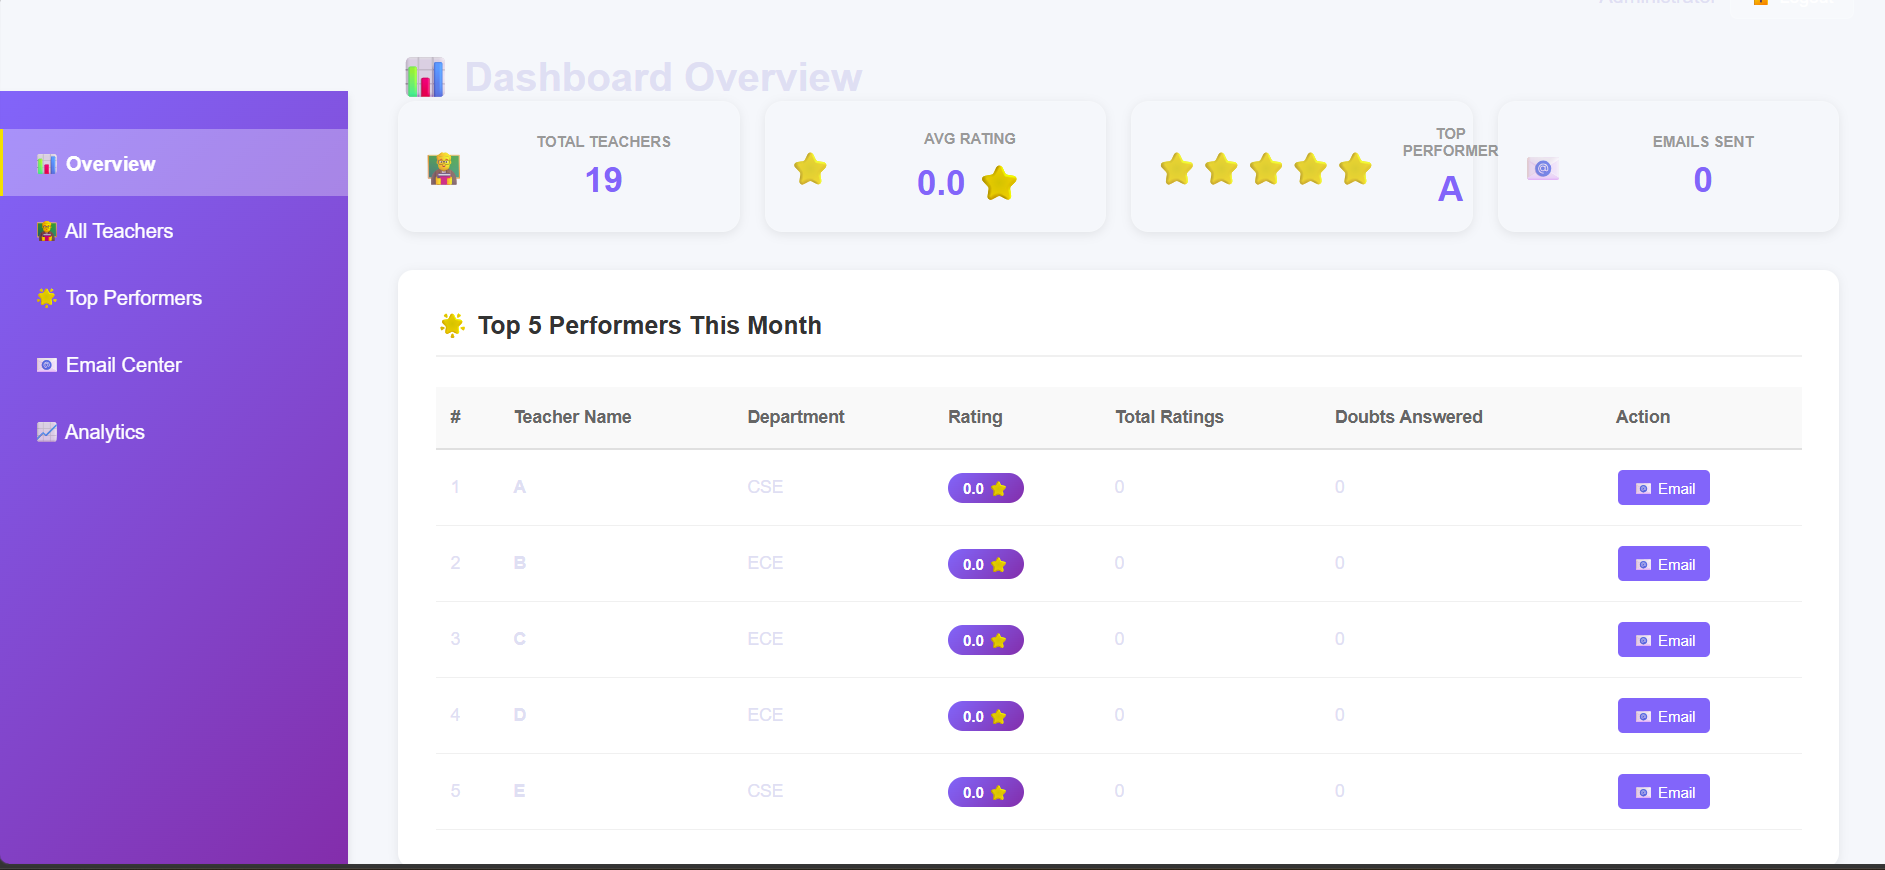
\includegraphics[width=0.95\textwidth]{screenshots/Admin-Dashboard.png}
\caption{Admin Dashboard with Analytics}
\end{figure}
\noindent\textit{The admin dashboard provides institutional-level performance monitoring. It integrates rankings, summary metrics, and communication controls for reporting.}

\section{Observed Results}
\begin{enumerate}[label=\Alph*., leftmargin=1.5em]
    \item Student feedback collection and professor rating functions operate correctly.
    \item Doubt posting constraints and response flow are operational.
    \item Prediction history and chart visualization are updated dynamically.
    \item Admin performance monitoring and email reporting are integrated.
\end{enumerate}

\section{Core Functional Outcomes}
\begin{enumerate}[label=\Alph*., leftmargin=1.5em]
    \item \textbf{Authentication:} Role-based redirection works reliably for all user categories.
    \item \textbf{Rating Workflow:} Professor-wise rating aggregation updates correctly after submissions.
    \item \textbf{Doubt Workflow:} Student-to-professor query lifecycle is completed with status visibility.
    \item \textbf{Prediction Module:} Multi-factor input successfully generates expected score output and trend records.
    \item \textbf{Admin Analytics:} Teacher performance ranking and bulk communication are operational.
\end{enumerate}

\section{Technical Achievement Highlights}
\begin{enumerate}[label=\Alph*., leftmargin=1.5em]
    \item Integration of frontend and backend modules with consistent role checks.
    \item Combined chart visualization with persisted prediction data.
    \item Reporting automation through email APIs.
    \item Readable and modular code organization for maintainability.
\end{enumerate}

\section*{Chapter Summary}
This chapter demonstrated the implementation outcomes through interface evidence, workflow verification, and functional observations. The presented screenshots and explanations confirm that the system behaves correctly across student, professor, and admin roles.


\chapter{Conclusion and Future Scope}
\section{Conclusion}
EduRate successfully delivers a complete role-based academic feedback and analytics system aligned with institute-level requirements. The project combines authentication, professor rating, doubt interaction, prediction support, and administrative communication within a single integrated workflow. The implemented architecture demonstrates that transparent faculty evaluation and student support can be handled efficiently through a modular web platform.

From an academic systems perspective, the project validates the practicality of integrating multiple institutional processes into one platform rather than maintaining disconnected tools. The rating workflow supports structured performance evidence, the doubt module improves student-faculty engagement continuity, and the analytics layer transforms raw records into meaningful decision support. The performance predictor further extends the system from retrospective feedback toward forward-looking student assistance.

Overall, the implementation fulfills its primary technical and functional goals by providing secure access control, maintainable architecture, and measurable output for key stakeholders. The final system is not only operational but also extensible, which is essential for long-term institute adoption and incremental feature evolution.

\section{Key Contributions}
\begin{itemize}[leftmargin=1.5em]
    \item Unified multi-role workflow for students, professors, and administrators.
    \item Actionable rating and doubt modules instead of static data collection.
    \item Student-side prediction support with trend visibility.
    \item Administrative performance analytics with email-based reporting.
\end{itemize}

\section{Future Scope}
\begin{itemize}[leftmargin=1.5em]
    \item Automated semester-wise report export in PDF format.
    \item AI-based sentiment analysis for text feedback.
    \item Notification system for doubt replies and admin announcements.
    \item Advanced predictive models and confidence intervals.
    \item Long-term department-level analytics dashboards.
\end{itemize}

\section{Final Remark}
This project establishes a practical foundation for data-driven academic quality monitoring and educational process transparency. By combining feedback capture, engagement workflows, and reporting in one unified system, EduRate demonstrates how software engineering can directly support academic governance and continuous improvement.

With incremental refinement in analytics depth, automation, and predictive intelligence, the platform can evolve into a comprehensive institutional decision-support environment. In its current form, the project already provides strong applied value for students, faculty, and administrators, while also leaving clear pathways for research and production-level enhancement.


% ===================== REFERENCES =====================
\nocite{*}
\bibliography{report}
\bibliographystyle{unsrt}

\end{document}
